\documentclass[conference]{IEEEtran}
\IEEEoverridecommandlockouts
% The preceding line is only needed to identify funding in the first footnote. If that is unneeded, please comment it out.
\usepackage{cite}
\usepackage{url}
\usepackage[english]{babel}
\usepackage{amsmath,amssymb,amsfonts}
\usepackage{algorithmic}
\usepackage{graphicx}
\graphicspath{ {./images/} }
\usepackage{textcomp}
\usepackage{xcolor}
\def\BibTeX{{\rm B\kern-.05em{\sc i\kern-.025em b}\kern-.08em
    T\kern-.1667em\lower.7ex\hbox{E}\kern-.125emX}}
\begin{document}

\title{Free-viewpoint video synthesis for soccer games\\
% {\footnotesize \textsuperscript{*}Note: Sub-titles are not captured in Xplore and
% should not be used}
% \thanks{Identify applicable funding agency here. If none, delete this.}
}

\author{\IEEEauthorblockN{Davide Lusuardi}
\IEEEauthorblockA{\textit{Department of information engineering and computer science} \\
\textit{University of Trento}\\
Trento, Italy \\
davide.lusuardi@studenti.unitn.it}
}

\maketitle

\begin{abstract}
In this paper, we present and discuss some methods for free-viewpoint synthesis for soccer games.
These techniques permit to generate novel views of actions from any angle and allow viewers to virtually fly through real soccer scenes.

% In this document, we discuss some methods to accomplish free-viewpoint video visualization for soccer scenes.
% These methods generate novel views of actions from any angle and allow viewers to virtually fly through real soccer scenes.
% TODO: complete
% and is of interest for visualization in TV productions.
\end{abstract}

% \begin{IEEEkeywords}
% component, formatting, style, styling, insert
% \end{IEEEkeywords}

\input{sec01_introduction.tex}
\input{sec02_overview.tex}

\section{The iview system}
In this section we present the \textit{iview} free-viewpoint video
system (www.bbc.co.uk/rd/iview) which enables the production of novel desirable camera views such as 
the goal keeper view, the referee view or even the ball camera.
This system exploits the already placed live TV broadcast cameras as the primary
source of multiple view video.
Usually football matches are covered by 12-20 high-definition cameras placed all over in the stadium
providing wide-baseline views.
Match cameras are manually controlled to follow the game play zooming in on events when occurs.
However, only a fraction of these are focused on specific events of interest and can be used for production 
of free-viewpoint renders, the remaining cameras cover the pitch, crowd and coaches.


% Robust algorithms are required for both recovery of camera
% calibration from the broadcast footage and wide-baseline correspondence between
% views for reconstruction or view interpolation.

% Therefore
% iview uses a method for real-time camera calibration from the match footage [2:46].
% Player segmentation is performed using chroma-key and difference matting tech-
% niques independently for each camera view [2:15]. Automatic calibration and player
% segmentation for moving broadcast cameras results in errors of the order of 1-3
% pixels which is often comparable to the size of players arms and legs in the broad-
% cast footage. Robust reconstruction and rendering of novel viewpoints is achieved in
% the iview system by an initial conservative visual-hull reconstruction followed by a
% view-dependent refinement. View-dependent refinement simultaneously refines the
% player reconstruction and segmentation exploiting visual cues from multiple cam-
% era views. This achieves free-viewpoint rendering with pixel accurate alignment of
% neighbouring views to render novel views with a visual quality approaching that
% of the source video.

% Advances are presented in real-time through the
% lens camera calibration to estimate both the camera pose, focus and lens distortion
% from the pitch marks.

% Free-viewpoint video is then produced starting with a volu-
% metric reconstruction followed by a view-dependent refinement using information
% from multiple views.

% Automatic online calibration, segmentation and reconstruction is performed to allow
% rendering of novel viewpoints from the moving match cameras.

\begin{figure}[htbp]
\centerline{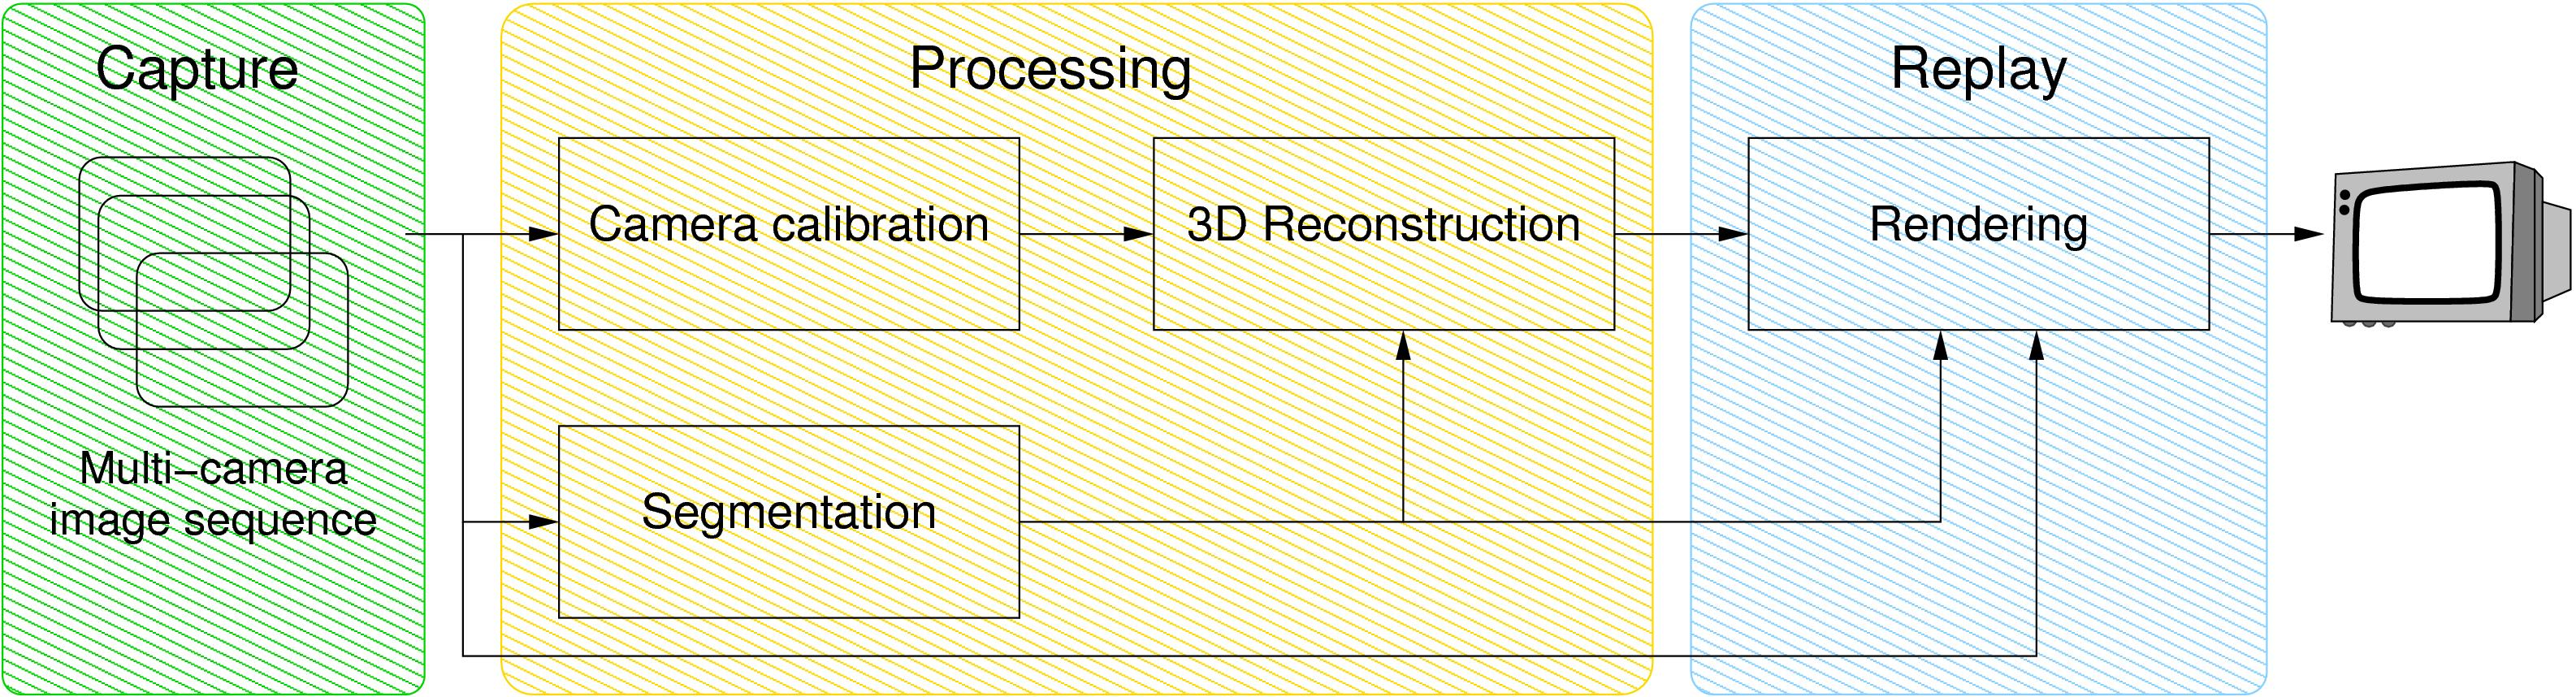
\includegraphics[scale=0.078]{iview_overview2.png}}
\caption{Overview of the free-viewpoint system. [TODO: cite 02.1]}
\label{fig:iview_overview}
\end{figure}


The \textit{iview} system is composed of three main modules as shown in Figure \ref{fig:iview_overview}: 
capture, processing, and replay module.

Capture is performed using time synchronised acquisition from both auxiliary and
match cameras.
The minimal number of cameras is about four, but for good quality results a higher number is required.
Camera synchronisation is achieved using standard genlock process.

The processing module computes a 3D model of the scene.
This is done using segmentation of objects from the back-
ground and 3D reconstruction \cite{iview2.1}.

In order to allow the use of footage from match cameras and to avoid the need for prior calibration, 
automatic calibration of all cameras is performed using a line-based approach againts the pitch lines of the captured footage, 
achieving a root-mean-square error of 1-2 pixels for moving cameras. 
The calibration is very fast and robust, capable of real-time operation for use during live match footage. 
Calibration estimates the extrinsic and intrinsic parameters of each camera including lens distortion.

The segmentation is needed to separate the foreground, i.e. the players from the background.
Matting of players from the green pitch is performed using chroma-keying matting. 
% This allows the approximate segmentation of the foreground players for subsequent processing to produce free-viewpoint video. 
The authors developed and tested a k-nearest neighbour approach for chroma-keying and evaluated two other known techniques,
\textit{Fast green subtraction} in RGB colour space and keying in HSV colour space.
The k-nearest neighbour classifier is controlled by a GUI where the user has to click on position in the image that correspond
to background. 
The process is repeated until the resulting segmentation is satisfying.
A deeper explanation is present in the paper \cite{iview2.1} where the authors present and evaluate also 
\textit{Fast green subtraction} and keying in HSV.



Aperture correction is also applied to each video sequence to correct for the camera edge enhancement
used in standard broadcast footage \cite{iview}.

% Likewise matting in relatively uncontrolled outdoor conditions with changing illu-
% mination achieves a segmentation within 1-2 pixels of the true foreground with the
% addition of background clutter for the crowd, hoardings and on-pitch advertising.





% The replay module renders the captured scene in realtime
% using the computed 3D model and the original camera images
% deploying view-dependent texture mapping [8].
% The entire system can potentially operate in real-time. At
% the current stage the processing is done offline. That means
% the images are stored and the processing is run at a later stage.
% The replay module is designed to work at interactive rates.
\section{Image-based rendering}

\begin{figure}[htbp]
\centerline{\includegraphics[scale=0.078]{plane_sweeping.png}}
\caption{Overview of the free-viewpoint system. [TODO: cite 02.1]}
\label{fig:plane_sweeping}
\end{figure}

In this section we present a different approach to FVV.
Instead of performing 3D reconstruction, image-based methods generate directly the image of the novel viewpoint.
When multiple cameras are present, plane sweeping can be used [05:Yang et al., 2004] for both small and wide 
baseline setups.
Plane sweeping has already been used for novel view point in soccer scenes. Goorts et al. [05:Goorts
et al., 2012a; Goorts et al., 2013a] present a method
with two plane sweeps and a depth filtering step suitable for smaller baseline 
setups of about 1 meter. 
Moreover, this method has some problems like disappearing players
if they overlap in the image.


\section{Billboard-based visualization}
In this section we present the work of Ohta et al. \cite{billboard}.
The authors use billboard representation to make a 3D model of each player.
This method is simpler than full 3D reconstruction and require less computation.
A player billboard is a small rectangle standing perpendicular to the ground
and a 2D texture is shown on it.
The difference between 3D reconstruction and billboard representation is shown in Figure \ref{fig:billboard_comparison}:
the visual difference is clear at a close viewpoint but becomes very small at a distant viewpoint.

\begin{figure}[htbp]
\centerline{\includegraphics[scale=0.22]{billboard_comparison.png}}
\caption{Appearance similarity between 3D reconstruction and billboard in close and distant view \cite{billboard}}
\label{fig:billboard_comparison}
\end{figure}

\input{sec06_conclusion.tex}



\bibliographystyle{IEEEtran}
\bibliography{biblio.bib}



\end{document}